\documentclass{article}
\usepackage[utf8]{inputenc}
\usepackage{amsmath}
\usepackage{amsthm}
\usepackage{amssymb}
\usepackage{float}
\usepackage{graphicx}
\usepackage{dirtytalk}
\usepackage{algorithm}
\usepackage{hyperref}
\usepackage[noend]{algpseudocode}
\graphicspath{ {./images/} }
\newtheorem{theorem}{Theorem}[section]
\theoremstyle{definition}
\newtheorem{definition}{Definition}[section]
\theoremstyle{remark}
\newtheorem*{remark}{Remark}
\newtheorem{lemma}[theorem]{Lemma}
\newenvironment{problem}[2][Example]{\begin{trivlist}
\item[\hskip \labelsep {\bfseries #1}\hskip \labelsep {\bfseries #2.}]}{\end{trivlist}}

\usepackage{biblatex}
\addbibresource{references.bib}

\title{Bifurcation Theory - Continuous and Discrete}
\author{Alan Chen, Byron Fan, Alex Mark}
\date{December 2021}

\begin{document}

\maketitle

\tableofcontents
\pagebreak
\section{Motivation and Background}
Essentially all simple ordinary differential equations (ODEs) appear in the following form:
\begin{equation}
    \frac{dx}{dt} = f(x, t)
\end{equation}
There exist a plethora of methods to analyze and solve these models, as we have witnessed in class, but unfortunately, most real life scenarios are nowhere near this simple. 

A complication that one might begin to consider is models in which there exist unknown potentially varying parameters in addition to just the dependent variable. For instance, one might be interested in the amount of hunting of deer that we can permit before there is irreversible damage to the species' population and the surrounding ecosystem. To analyze this problem, one might consider constructing a model that has a right-hand-side (RHS) dependent not only the population of deer but also a parameter for the hunting rate $h$. Then, in the analysis, we would have to investigate how the population changes over time given different values of $h$. 

Another example that was given in class involved a climate model that modeled the temperature of the Earth. The main extra parameter that was of interest was the impact of greenhouse gases on the emission of energy from the Earth. With this model, we can then perform very useful and meaningful analysis on how greenhouse gases can impact the temperature of the Earth.    

Clearly, these "extra parameter" models have several important applications that motivate the formalization of their study into an entire field called \textbf{bifurcation theory}. Simply put, in bifurcation theory, we attempt to study differential equations (or difference equations in the discrete case, as we will see later) that have extra parameters that can be varied in addition to the dependent variable. Notably, we would like to see how these extra parameters affect the behavior of the solutions to the differential/difference equations and then make conclusions based off of this behavior. 

In this paper, we will cover introductory formalisms of bifurcation theory, common bifurcations, and discretized versions with their properties.

\section{Introduction to Bifurcations}
More formally, we can begin to consider the following types of autonomous ODEs:
\begin{equation}\label{bf ode}
    \frac{dx}{dt} = f(x, \alpha_1, \alpha_2, ..., \alpha_n)
\end{equation}
\begin{definition}[Bifurcation Parameter]
    In an ODE of the form of Eq. \ref{bf ode}, $\alpha_j \forall j \in \{1, 2, ..., n\}$ are the \textbf{bifurcation parameters}. The number of bifurcation parameters in an ODE determines its classification: Eq. \ref{bf ode} is known as a \textbf{n-parameter map}.
\end{definition}
For our purposes, we will mainly focus on the $n = 1$ case or one-parameter maps, as they provide sufficiently interesting material to cover, but it is important to note the existence of $n > 1$ parameter maps that can arise in more complex modeling scenarios. 
\begin{remark}
On the other hand, we would like to point out that it is often useful to reduce $n > 1$ parameter maps to $n = 1$ parameter maps, as we can then analyze each parameter independent of the others to see its isolated effect on the dependent variable of interest. 
\end{remark}


% probably have figures illustrating a bifurcation: one showing a stable equilibria under alpha = something, and another showing the same equilibria but unstable under alpha = another thing

\subsection{General Approach}
The following steps outline the general approach to analyzing problems involving bifurcation parameters.  
\begin{enumerate}
    \item Calculate the equilibria w.r.t the bifurcation parameter.
    \item Perturb the system near the equilibria to determine stability.
    \item Draw conclusions about system's behavior based on \textbf{bifurcation plots}.
\end{enumerate}

We illustrate this process by working through the following example, which will also reveal the first commonly observed bifurcation.
\subsection{Saddle Node Bifurcation}
\begin{problem}{2.1.1}
Perform a qualitative analysis of the following differential equation:
\begin{equation}\label{example 2.1}
    \frac{dx}{dt} = -x^2 + \alpha .
\end{equation}
\end{problem}
\begin{proof}[Solution]\renewcommand{\qedsymbol}{}
Following the process illustrated above, the first step is to find the equilibria of the differential equation. This occurs when the LHS is $0$:
\begin{align}\label{equilibria 2.1}
    \frac{dx}{dt} &= 0 = -x^2 + \alpha \nonumber
    \\
    \implies x &= \boxed{\pm \sqrt{\alpha}}
\end{align}

Notice that our solutions are now dependent on $\alpha$! So, instead of a single point like with simple ODEs, when plotted on the $x$-$\alpha$ plane, we have an infinite set of equilibria. 

The next step is figuring out how the solutions behave outside of these equilibria. Of course, we can use the methods discussed in class, but we introduce another way to think about this concept that may be easier when approaching specifically bifurcation problems. 

We want to perturb around the solutions in (\ref{equilibria 2.1}). For simplicity, let's call the equilibria $x_\epsilon$, and consider how we can describe a perturbation:
\begin{equation}
    x = x_\epsilon \pm \Delta x(t)    
\end{equation}
where $\Delta x(t)$ is a very small number that has $t$ dependence.

We can plug this back into the differential equation in Eq. \ref{example 2.1}, where the LHS simplifies to 
\begin{equation*}
    \frac{d(x_\epsilon + \Delta x)}{dt} = \frac{d\Delta x}{dt}
\end{equation*}
since $x_\epsilon$ is a constant, and the RHS simplifies to 
\begin{align*}
    -x^2 + \alpha &= -(x_\epsilon + \Delta x)^2 + \alpha \\
    &= -x_\epsilon^2 - 2x_\epsilon\Delta x - \Delta x^2 + \alpha \\
    &= -\alpha - 2x_\epsilon\Delta x - 0 + \alpha \\
    &= -2x_\epsilon\Delta x.
\end{align*}
Thus, giving us the following differential equation to solve:
\begin{equation}
    \frac{d\Delta x}{dt} = -2x_\epsilon\Delta x
\end{equation}
which is easily solvable through a variety of methods - linear, separable, qualitative, etc. No matter how we choose to do it, we arrive at the solution:
\begin{equation*}
    \Delta x(t) = \boxed{\Delta x_0 e^{-2x_\epsilon t}}
\end{equation*}
where $\Delta x_0$ is some constant trivially solvable through plugging in the initial condition @ $t = 0$. Taking a closer look at this equation, we can observe the following:
$$
\lim_{t\to\infty}\Delta x(t) = 
\left\{ 
    \begin{array}{ll}
        0 & \mbox{if $x_\epsilon > 0$} \implies \text{stable},  \\
        \infty & \mbox{if $x_\epsilon < 0$} \implies \text{unstable} \\
    \end{array}
\right. \\
$$

Therefore, we arrive at the following \textbf{bifurcation diagram}, where the $\alpha$-axis runs horizontally and the $x$-axis runs vertically:
\begin{figure}[H]
    \centering
    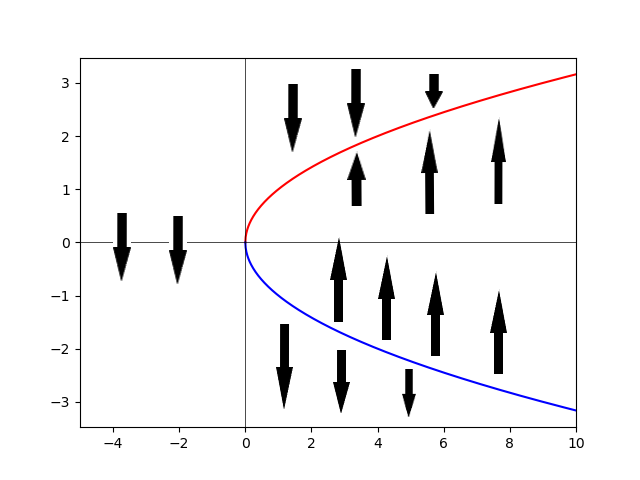
\includegraphics[width=80mm,scale=0.5]{images/Saddle.png}
    \caption{Bifurcation diagram of Example 2.1. Note the differing stability around the two equilibrium curves.}
    \label{fig:saddle}
\end{figure}
\end{proof}

\begin{definition}
    This example illustrates an extremely common bifurcation called the \textbf{saddle-node bifurcation}.
\end{definition}
Saddle-node bifurcations are typically used in reference to continuous dynamical systems. As seen above, our solution to equation (3) finds that we have a stable and unstable branch that start from (0,0). 

Now, we analyze the stability structure of the saddle node. In Figure 1, the red line towards $x_\epsilon$ = $\sqrt{\alpha}$ displays a stable branch since all solutions are pointing towards it around that line. For the blue line, all solutions are moving away from that line so it is an unstable branch. When $x_\epsilon$ $<$ 0, there are no equilibrium solutions, so all solutions are moving toward  $-\infty$. 

Saddle node bifurcations appear everywhere, though extremely commonly in physics where quadratic relationships appear often, such as with controlling voltage and preventing overloading \cite{Dobson1992}. 

We will now visit the zoo of bifurcations and explore a few common ones in a similar manner. 
\subsection{Transcritical Bifurcation}
\begin{problem}{2.3.1}
If we modify equation (3) slightly, we have the following differential equation: 
\begin{equation}\label{example 2.3}
    \frac{dx}{dt} = -x^2 + \alpha x .
\end{equation}
\end{problem}

\begin{proof}[Solution]\renewcommand{\qedsymbol}{}
In this differential equation, the parameter $\alpha$ changes dynamics. Using the same process as before, we find the equilibrium solutions:
\begin{align}\label{equilibria 2.3}
    &\frac{dx}{dt} = 0 = 
    x(\alpha - x) \nonumber 
    \\
    \implies &x_\epsilon = \boxed{0, \alpha}
\end{align}

Again, we want to perturb around the equilibrium using the following:
\begin{equation}
    x = \boxed{x_\epsilon \pm \Delta x(t)} 
\end{equation}

As such, we find the following differential equation: 
\begin{equation}
    \frac{d\Delta x}{dt} = \alpha \Delta x -2x_\epsilon \Delta x
\end{equation}

which is a linear differential equation, so we arrive at the solution: 

\begin{equation}
    \Delta x(t) = \boxed{\Delta x_0  e^{(\alpha - 2 x_\epsilon)t}}
\end{equation}

\begin{figure}[H]
    \centering
    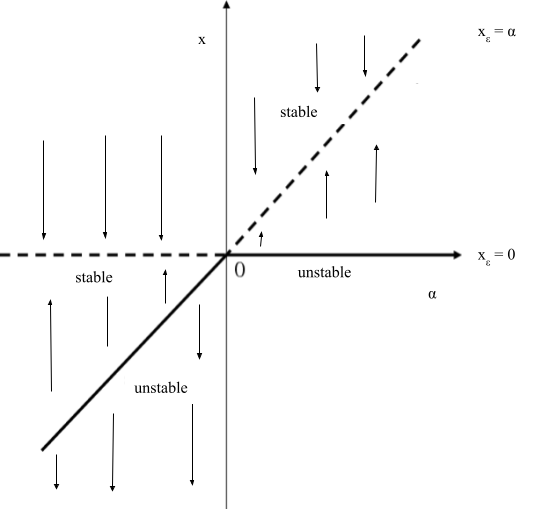
\includegraphics[width=80mm,scale=0.5]{images/Transcritical.png}
    \caption{Bifurcation diagram of Example 2.3. Note the stability exchange at $\alpha = 0$.}
    \label{fig:transcritical}
\end{figure}
\end{proof}

\begin{definition}
    This example illustrates a particular local bifurcation called the \textbf{transcritical bifurcation}.
\end{definition}
Transcritical  bifurcation is a special kind of local bifurcation that is characterized having a eigenvalue with the real part passing through zero for the equilibrium \cite{Roesch2019}. 

In Figure 2, we observe that there are two lines, $x_\epsilon$ = $0$ and $x_\epsilon$ = $\alpha$. There is a transition of stability as $\alpha$ changes from negative to positive, which is the transcritical bifurcation. So, $x_\epsilon$ = $\alpha$ equilibrium solution is unstable from $\alpha$ = ($-\infty$,0) and stable from $\alpha$ = (0,$\infty$). The $x_\epsilon$ = $0$ equilibrium solution is stable from $\alpha$ = ($-\infty$,0) and unstable from $\alpha$ = (0,$\infty$). Thus, the bifurcation point is at $\alpha$ = 0. 
\subsection{Pitchfork Bifurcation}
\begin{problem}{2.4.1}
If we modify equation (7) by replacing $x^2$ with $x^3$, we have another interesting differential equation: 
\begin{equation}\label{example 2.4}
    \frac{dx}{dt} = -x^3 + \alpha x .
\end{equation}
\end{problem}

\begin{proof}[Solution]\renewcommand{\qedsymbol}{}
In this differential equation, the parameter $\alpha$ changes dynamics, but now we have $x^3$. Using the same process as before, we find the equilibrium solutions:
\begin{align*}\label{equilibria 2.4}
    &\frac{dx}{dt} = 0 = 
    x(\alpha - x^2) \nonumber 
    \\
    \implies &x_\epsilon = \boxed{0,\pm \sqrt{\alpha}}
\end{align*}

We want to perturb around the equilibrium using the following:
\begin{equation}
    x = \boxed{x_\epsilon \pm \Delta x(t)} 
\end{equation}

Therefore, we obtain the following differential equation: 
\begin{equation}
    \frac{d\Delta x}{dt} = (\alpha - 3 x_\epsilon ^2) \Delta x
\end{equation}

this is the representation of the linear stability around $x_\epsilon$, so we arrive at the solution:

\begin{equation}
    \Delta x(t) = \boxed{\Delta x_0  e^{(\alpha - 3 x_\epsilon^2)t}}
\end{equation}

From this solution, we look at the exponent term to evaluate when it is positive or negative for each of the three branches. 

\begin{figure}[H]
    \centering
    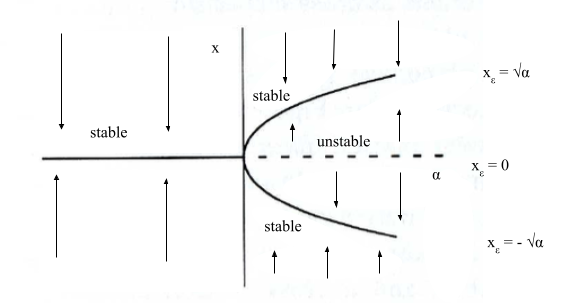
\includegraphics[width=115mm,scale=1.0]{images/Pitchfork.png}
    \caption{Bifurcation diagram of Example 2.4. Note the stability of the three branches starting from $\alpha = 0$.}
    \label{fig:pitchfork}
\end{figure}
\end{proof}

\begin{definition}
    This example illustrates the \textbf{pitchfork bifurcation}.
\end{definition}
The pitchfork bifurcation is another type of local bifurcation, but the system transitions from one node to three fixed points. In this analysis, we will focus on the supercritical case since our differential equation is presented in the normal form of the supercritical pitchfork bifurcation \cite{Balibrea2010}.

In Figure 3, we observe that there are three branches in our bifurcation diagram: $x_\epsilon$ = $\sqrt{\alpha}$, $x_\epsilon$ = $0$, $x_\epsilon$ = $-\sqrt{\alpha}$. By following the stability structure of the pitchfork node, we observe an interesting pattern. 

When $\alpha$ $<$ 0, only the $x_\epsilon$ = $0$ branch exists, and is stable as solutions collapse towards 0. However, we soon as we reach $\alpha$ = 0, there are three branches, where the $x_\epsilon$ = $0$ branch becomes unstable while the $x_\epsilon$ = $\pm \sqrt{\alpha}$ solution branches are stable. Therefore, the diagram shows that our pitchfork bifurcation leads to solutions of $x_\epsilon$ = $\sqrt{\alpha}$ when $x_\epsilon$ $>$ 0, and $x_\epsilon$ = $-\sqrt{\alpha}$ when $x_\epsilon$ $<$ 0.
\subsection{Hopf Bifurcation}
\begin{problem}{2.5.1}
We now consider systems with two differential equations that are nonlinear.   
\begin{align}\label{example 2.5}
    \frac{dx}{dt} = -y + (\alpha - x^2 -y^2)x 
    \\
    \frac{dy}{dt} = x+ (\alpha - x^2 -y^2)y
\end{align}
\end{problem}

\begin{proof}[Solution]\renewcommand{\qedsymbol}{}
In this new system, we have two nonlinear differential equations  
\begin{align}\label{equilibria 2.5}
    \frac{dx}{dt} = 0 = 
   -y + (\alpha - x^2 -y^2)x \nonumber 
    \\
    \frac{dx}{dt} = 0 = 
    x+ (\alpha - x^2 -y^2)y \nonumber
\end{align}


We want to perturb around the equilibrium solution. First, we perturb around the origin:
\begin{align}
    x = \boxed{0 \pm \Delta x(t)}
    \\
    y = \boxed{0 \pm \Delta y(t)} 
\end{align}

Therefore, we obtain the following differential equation system: 
\begin{align}
    \frac{d\Delta x}{dt} = -\Delta y + \alpha \Delta x
    \\
    \frac{d\Delta y}{dt} = \Delta x + \alpha \Delta y
\end{align}

Then, we rewrite these equations as a system of differential equations. 

\[\frac{dx}{dt} = 
\begin{vmatrix}
\alpha & -1\\
1 & \alpha
\end{vmatrix} x\]

Then, evaluating the matrix helps find the eigenvalues similar to the phase plane analysis procedures from class. 

Thus, we find the eigenvalues:
\begin{equation}
    \lambda_\pm = \alpha \pm i
\end{equation}

Notice that there is an imaginary part, which tells us the solutions are oscillating with frequency 1. Additionally, $\alpha$ tells us that if it is positive, we have exponential growth, and if it is negative, we have exponential decay. Therefore, our stability is completely dependent on the value of $\alpha$.

A simpler way to represent this differential equation is to use a system of differential equations using polar coordinates.

%insert coordinate transformation
\begin{equation}
    \frac{dr}{dt} = r(\alpha-r^2)
\end{equation}

\begin{equation}
    \frac{d\theta}{dt} = 1
\end{equation}

This coordinate transformation leads to the solution:

\begin{equation}
    \theta = t + \theta_\epsilon
\end{equation}

\begin{equation}
    r^2 = \begin{cases} \alpha r^2_\epsilon / r^2_\epsilon + (\alpha-r^2_\epsilon)e^{-2\alpha t}, & \mbox{if } \alpha{  \neq 0} \\ r^2_\epsilon / (1 + 2r^2_\epsilon t), & \mbox{if } \alpha \mbox{= 0} \end{cases}
\end{equation} 

From this solution, we have a 3-D graphical representation of the differential equations system.

\begin{figure}[H]
    \centering
    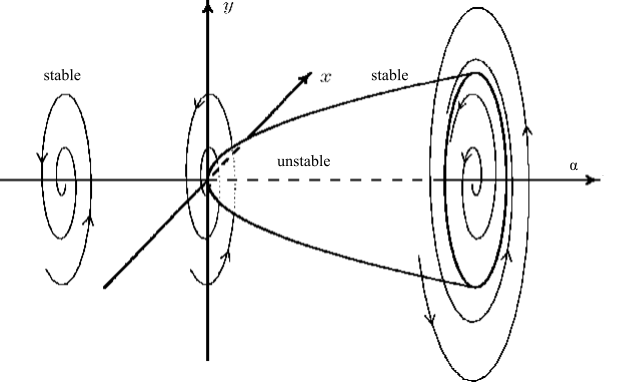
\includegraphics[width=100mm,scale=1.0]{images/Hopf.png}
    \caption{Bifurcation diagram of Example 2.5. Note the differing stability based on the value of $\alpha$ from our solution. Image obtained from Navarro et al. \cite{Navarro2008}}
    \label{fig:hopf}
\end{figure}
\end{proof}

\begin{definition}
    This example illustrates the \textbf{Hopf bifurcation}.
\end{definition}
The Hopf bifurcation is a fascinating type of local bifurcation. There is a critical fixed point that results in the dynamical system losing stability given the pair of complex conjugate eigenvalues from the cross into the complex plane imaginary axis. This is illustrated by a periodic solution surrounding the equilibrium point either arising and going away as $\alpha$ varies.

In Figure 4, we observe that the three axes are x, y, and $\alpha$. In this analysis, we focus on the effects from the positive and negative values of $\alpha$. 

When $\alpha < 0$, the graph  spirals in to the solution at $0$, so it's stable. However, when the bifurcation point is passed so that $\alpha > 0$, the cylindrical coordinates present another branch of solutions. The $\alpha = 0$ becomes unstable and the solution oscillates away from the origin as $r = \alpha$ grows. Using polar coordinates, we have $\frac{dr}{dt} = 0$, such that the solutions present a stable, cycling effect around that branch. Hopf bifurcations are instability that result in oscillations occurring at the bifurcation point. This is due to two eigenvalues cross from the left half plane to the right half plane of instability at characteristic frequencies, which can be seen as the cycles when $\alpha > 0$ in the figure above.

In this section, we have presented four main examples of bifurcations. It is important to recognize that given a dynamical system with parameters, the behavior of the solutions can change based on those parameters, which we have shown by perturbing around the transition points to characterize the type of bifurcation that occurs at these points.

\section{Discrete Bifurcation Theory}\label{dbt}
Currently, our definition of bifurcations and differential equations in general revolves around the central assumption of working in a continuous plane, which allows the LHS $\frac{dx}{dt}$ to make sense. However, there is a number of reasons why one might want to investigate a scenario where this assumption falls apart. 

The main motivation for discrete representations is that computers cannot process infinite, continuous data and instead approximate continuous data through a lot of small discrete intervals. So, computationally, we need a way to describe Eq. \ref{bf ode} in a discrete way. Alternatively, one might be interested in working with a domain that can only assume certain values. For example, a population of pandas can never be a non-integral value, so we could potentially be working with an axis that only has points $\in \mathbb{Z}^+$! 

We will hand-wave this section a bit, but the intuition is relatively straightforward. Interpreting the LHS' derivative as a slope, we define the following to be the analogous discrete version of Eq. \ref{bf ode}:
\begin{equation}\label{discrete bf ode}
    x_{t+1} = f(x_t, \alpha_1, \alpha_2, ..., \alpha_n)
\end{equation}
\begin{definition}[Difference Equation]
    Eq. \ref{discrete bf ode} is called a \textbf{difference equation} (very similar to differential equation!). 
\end{definition}
In essence, we are describing the next point as a function of the current point, which is exactly the information that a continuous slope tells us. However, it is completely done in discrete time, as the values of the function only assume $x_1, ... x_t$, a finite set as we only consider $t \in \{ 1, 2, ... \}$ without loss of generality. 
\subsection{Example - Logistic Map}\label{logmap}
An illustrative example of difference equations is the following relationship:
\begin{equation}\label{logisticEQ}
    x_{t+1} = f(x_t, r) = rx_t(1 - x_t)
\end{equation}
We would immediately like to point out the similarities to the logistic equation studied in class; the right hand side is essentially identical. 

This model has a lot of applications, a majority of which mainly only consider $r$ values between $[0, 4]$, since $\max(x_t(1 - x_t))$ if $x_t \in [0, 1]$ is $\frac{1}{4}$ which thus allows us to also bound $x_{t+1}$ between $[0, 1]$. 

Similar to before, we can consider how this model behaves given different values of $r$. We leave the discovery of the behavior as an exercise to the reader, but the key findings are summarized in Table \ref{table:logistictable} \cite{Yamagishi1997}.
\begin{table}[h!]
\centering
    \begin{tabular}{| c | c |} 
     \hline
     $r$ & Behavior \\ [0.5ex] 
     \hline \hline
     $(0, 1)$ &  $ \lim\limits_{t\to\infty} x_t =0$ \\ \hline
     $(1, 3)$ &  $ \lim\limits_{t\to\infty} x_t = \frac{r - 1}{r}$\\\hline
     $(3, 1 + \sqrt{6})$ & oscillation between $2$ points \\\hline
     $(1 + \sqrt{6}, \sim3.54409)$ & oscillation between $4$ points \\\hline
     $(\sim3.54409, 4)$ & oscillation between $2^k$ points for $k \geq 3$ \\ \hline
     $(4, \infty)$ & divergence to $|x_t| > 1$ \\[1ex]
     \hline
    \end{tabular}
    \caption{Results of bifurcation analysis on the logistic map difference equation.}
    \label{table:logistictable}
\end{table}

There is a lot of interesting behavior going on in Table \ref{table:logistictable} that we will discuss in the next section, especially for the oscillatory behavior for $r \in (3, 4)$. As aforementioned, the logistic map has numerous applications, the most notable being in modeling populations in ecology, sociology, and biology \cite{May1976}.
\subsection{Feigenbaum Constant}
Looking at Table \ref{table:logistictable} closely, we note the unique behavior between $r \in (3, 4)$, in which the oscillation progressively oscillates between more and more points. In particular, if we consider the values of $r$ for which the period \textbf{doubles}, or oscillates between $2^{k+1}$ points, the ratio of the distance between the critical points in which this occurs approaches the \textbf{first Feigenbaum Constant}, first discovered by physicist Mitchell J. Feigenbaum \cite{Feigenbaum1978}:
\begin{equation}
    \boxed{\delta \approx 4.669201...}
\end{equation}

Initially, Feigenbaum first observed this amazing result with respect to the logistic map described in Section \ref{logmap}, but it has since been conjectured and proved to hold for all one dimensional maps with a singular quadratic maximum \cite{Lanford1982, Tabor1989}. This is incredible, especially for its numerous applications, as that means that all of these maps bifurcate, or change behavior, at the same rate dictated by $\delta$.

Approximating and computing the Feigenbaum constant is a difficult problem of computational power, as it requires fine handling of floating point arithmetic and various precision techniques. It has proved to be an impressively interesting problem, comparable to the fanaticism with approximating $\pi$. One such method is outlined in the next section.
\subsection{Approximating Feigenbaum}
\cite{Briggs1991} outlines the ideas that form the core of all algorithms that approximate Feigenbaum's first constant. In this paper, we will only consider the following RHS of a difference equation, but note that the process can be generalized:
\begin{equation}\label{feigenbaumex}
    f_\alpha(x) = \alpha - x^2
\end{equation}
which should appear reminiscent of the saddle point bifurcation example (Eq. \ref{example 2.1}).

\begin{definition}($n$-cycle)
    An $n$-cyclic sequence is a sequence with an asymptotic period of oscillation of $n$. 
\end{definition}
As mentioned earlier, for Feigenbaum, we care about the $\alpha$s where the period doubles, or all functions where we have $n = 2^i$ for some $i$.

First, consider a set of recursive polynomials defined in the following manner:
\begin{equation}\label{bkdef}
    b_k(\alpha) = \alpha - [b_{k-1}(\alpha)]^2 \\
\end{equation}
\begin{equation}
    b_0(\alpha) = 0
\end{equation}

The method is based on the following lemma, which is claimed to be \say{trivial to prove}:
\begin{lemma}
    \textit{Let $k = 2^n$. Then $f_\alpha$ has a $k$-cycle if and only if $b_k(\alpha) = 0$.}
\end{lemma}
We believe this conclusion may not be immediately obvious, so we offer the following brief intuition for why it makes sense and how one might go about proving the result. 
\begin{proof}[Proof (Handwave)]
     Notice how $b_k$ is defined. The definition in Eq. \ref{bkdef} reminds us of how the original map was defined in Eq. \ref{feigenbaumex}; in fact, we point out that it is essentially identical. 
     
     We can use the analogous derivative/difference logic that was introduced in Section \ref{dbt} to interpret this fact: since $b_k$ is imitating the behavior of the derivative/difference of the solution, $b_k(\alpha) = 0$ implies that there is no change from the current time step to the next i.e. in the continuous case, the slope is $0$.
     
     Each location where the derivative is $0$, as we know by the first derivative test, represents either a local maxima or minima (though all we care about is that, notably, the direction changes). All points where this occurs, we observe, are the points that we count toward the $k$ points in the $k$-cycle. Therefore, finding the zeroes of $b_k$ is equivalent to finding the points in the $k$-cycle of Eq. \ref{feigenbaumex}. 
\end{proof}

The algorithm is outlined in Algorithm \ref{alg:approxfeigen}.
% http://keithbriggs.info/documents/how-to-calc.pdf

\begin{algorithm}[h!]
    \caption{Approximating Feigenbaum's first constant}\label{alg:approxfeigen}
    \begin{algorithmic}[1]
    \State $\alpha_0 \gets 0$ \Comment{Initial values}
    \State $\alpha_1 \gets 1$ 
    \State $\delta_1 \gets ~3.2$
    \State $i \gets 2$
    \While {i $\leq$ iterations}
        \State $x_0 \gets \alpha_{i-1} + \frac{\alpha_{i-1} - \alpha_{i-2}}{\delta_{i - 1}}$\vskip 3pt
        \State $\text{zero} \gets \textrm{newton}(b_{2^i}, x_0)$\vskip 3pt
        \State $\delta_i \gets \frac{\alpha_{i - 1} - \alpha_{i - 2}}{\alpha_{i} - \alpha{i - 1}}$\vskip 3pt
        \State $i \gets i + 1$
    \EndWhile
    \State \textbf{end} 
    \State $\delta = \lim_{i\to\infty}\delta_i$
    \end{algorithmic}
\end{algorithm}

Unfortunately, we do not have access to computers/programs that are efficiently and precisely able to approximate the zeroes of extremely high degree polynomials with finely spaced roots, as this is the key limitation of this algorithm. Notice that this is absolutely crucial, as the algorithm requires we determine the \textit{correct} zero according to the initial $x_0$, not just all of them. However, variants all based on this core algorithm have been used to approximate the Feigenbaum constant to thousands of decimal places \cite{Briggs1991}. 
\section{Concluding Remarks}
To study Bifurcation Theory is to study the chaos that resides in all aspects of life. From a young age, we are taught about the butterfly effect, which is the idea that small changes in an initial condition lead to drastically different outcomes. When dealing with both continuous and discrete maps, small changes (perturbations) to the initial conditions were made to analyze the behavior of such systems. Computational tools were then used to model the evolution of the iterated values. The concepts and methods discussed in this paper have many real world applications, some of which may not be immediately obvious. For example, the logistic map is ubiquitous throughout nature. As explored by Shaw in \cite{RS}, the behavior of a dripping faucet can be modeled by the logistic map as a function of water pressure, where the number of drops of water that occur double repeatedly until chaos is reached. This chaos served as inspiration for pseudo-random number generators, in which deterministic functions output seemingly unpredictable values. As expressed by May in \cite{May1976}, it would be beneficial for the general public if everyone understood the beauty behind simple equations such as the logistic map, and the important dynamical properties they hold.

\pagebreak

\printbibliography


\end{document}
